% \vspace{-.1cm}
\section{Experimental Evaluation}
\label{sec:experiments}

The focus of our experiments is to evaluate \method on the capabilities we would like from a data-driven planner.
In particular, we evaluate
\textbf{(1)} the ability to plan over long horizons without manual reward shaping,
\textbf{(2)} the ability to generalize to new configurations of goals unseen during training, and
\textbf{(3)} the ability to recover an effective controller from heterogeneous data of varying quality.
We conclude by studying practical runtime considerations of diffusion-based planning, including the most effective ways of speeding up the planning procedure while suffering minimally in terms of performance.

\subsection{Long Horizon Multi-Task Planning}
\label{sec:maze2d}

We evaluate long-horizon planning in the Maze2D environments \citep{fu2020d4rl}, which require traversing to a goal location where a reward of 1 is given.
No reward shaping is provided at any other location.
Because it can take hundreds of steps to reach the goal location, 
even the best model-free algorithms struggle to adequately perform credit assignment and reliably reach the goal (Table~\ref{table:maze2d}).

We plan with \method using the inpainting strategy to condition on a start and goal location.
(The goal location is also available to the model-free methods; it is identifiable by being the only state in the dataset with non-zero reward.)
We then use the sampled trajectory as an open-loop plan.
\method achieves scores over 100 in all maze sizes, indicating that it outperforms a reference expert policy.
We visualize the reverse diffusion process generating \method's plans in Figure~\ref{fig:maze2d}.

While the training data in Maze2D is undirected -- consisting of a controller navigating to and from randomly selected locations -- the evaluation is single-task in that the goal is always the same.
In order to test multi-task flexibility, we modify the environment to randomize the goal location at the beginning of each episode.
This setting is denoted as Multi2D in Table~\ref{table:maze2d}.
\method{} is naturally a multi-task planner; we do not need to retrain the model from the single-task experiments and simply change the conditioning goal.
As a result, \method{} performs as well in the multi-task setting as in the single-task setting.
In contrast, there is a substantial performance drop of the best model-free algorithm in the single-task setting (IQL; \citealt{kostrikov2021implicit}) when adapted to the multi-task setting.
Details of our multi-task IQL with hindsight experience relabeling \citep{andrychowicz2017hindsight} are provided in Appendix~\ref{app:multitask}.
MPPI uses the ground-truth dynamics; its poor performance compared to the learned planning algorithm of Diffuser highlights the difficulty posed by long-horizon planning even when there are no prediction inaccuracies.

\begin{figure}[t!]
\begin{flushright}
    % \raisebox{8.5\height}{\textbf{a}}
    \raisebox{.35\height}{\rotatebox{90}{\textbf{U-Maze}}}\hspace*{\fill}
    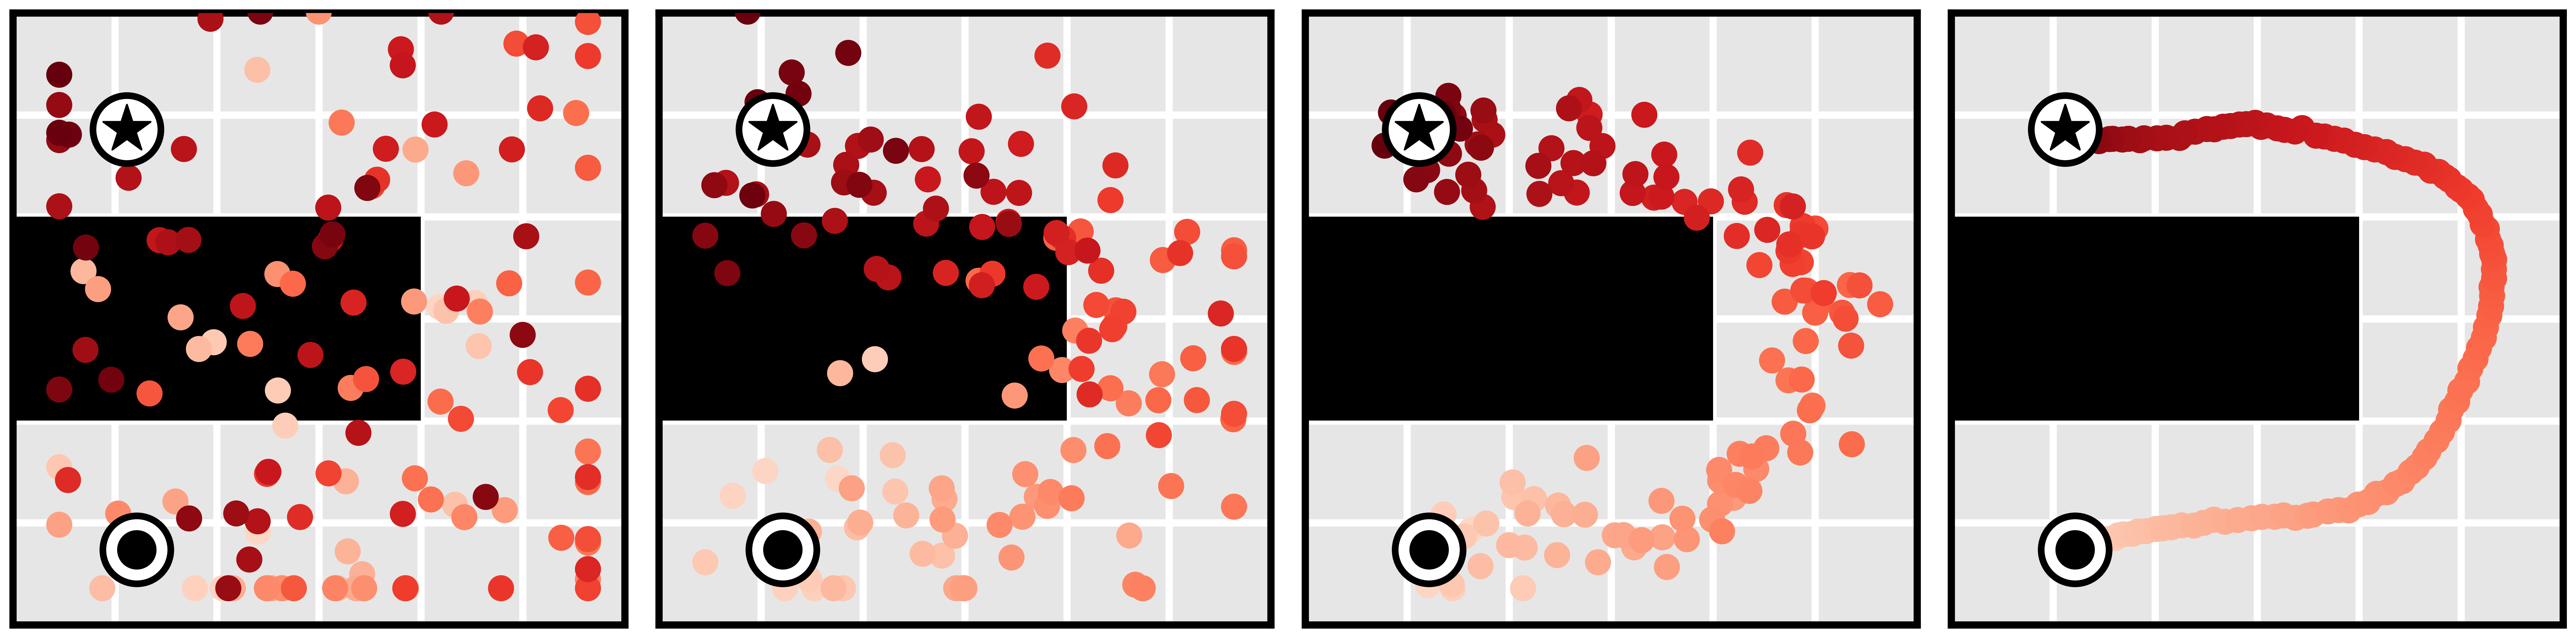
\includegraphics[width=0.95\columnwidth]{images/maze2d/maze2d-umaze-v1.png} \\
    %%
    % \raisebox{6.5\height}{\textbf{b}}
    \raisebox{.3\height}{\rotatebox{90}{\textbf{Medium}}}\hspace*{\fill}
    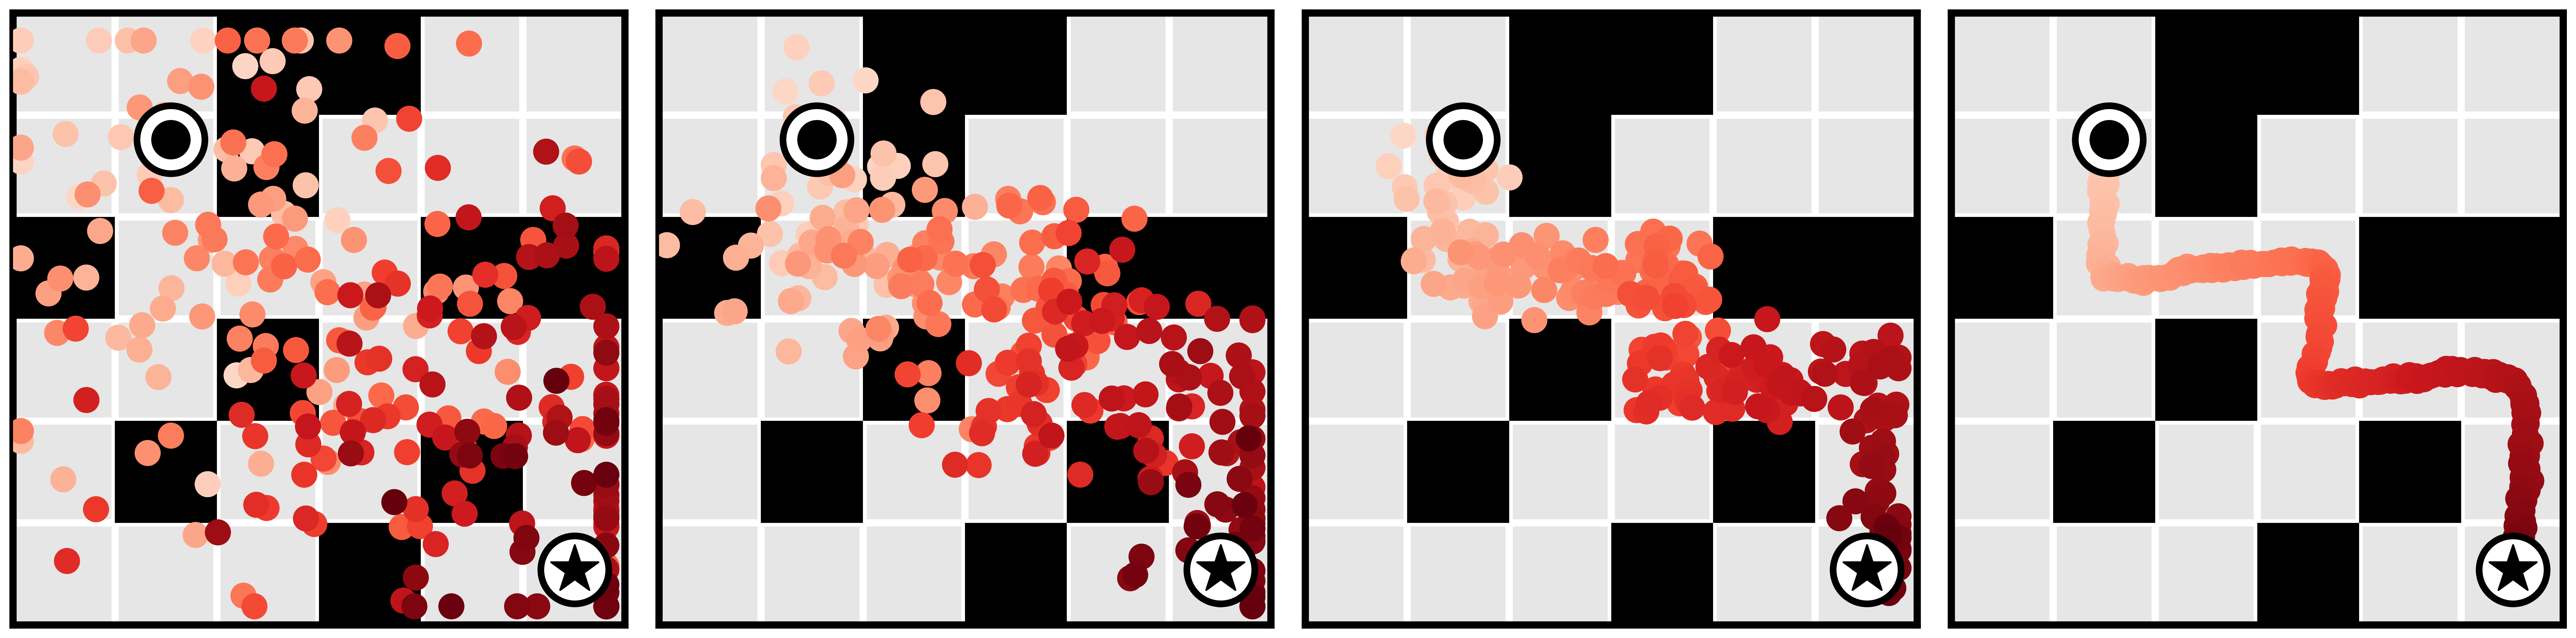
\includegraphics[width=0.95\columnwidth]{images/maze2d/maze2d-medium-v1.png} \\
    %%
    % \raisebox{8.5\height}{\textbf{c}}
    \raisebox{.6\height}{\rotatebox{90}{\textbf{Large}}}\hspace*{\fill}
    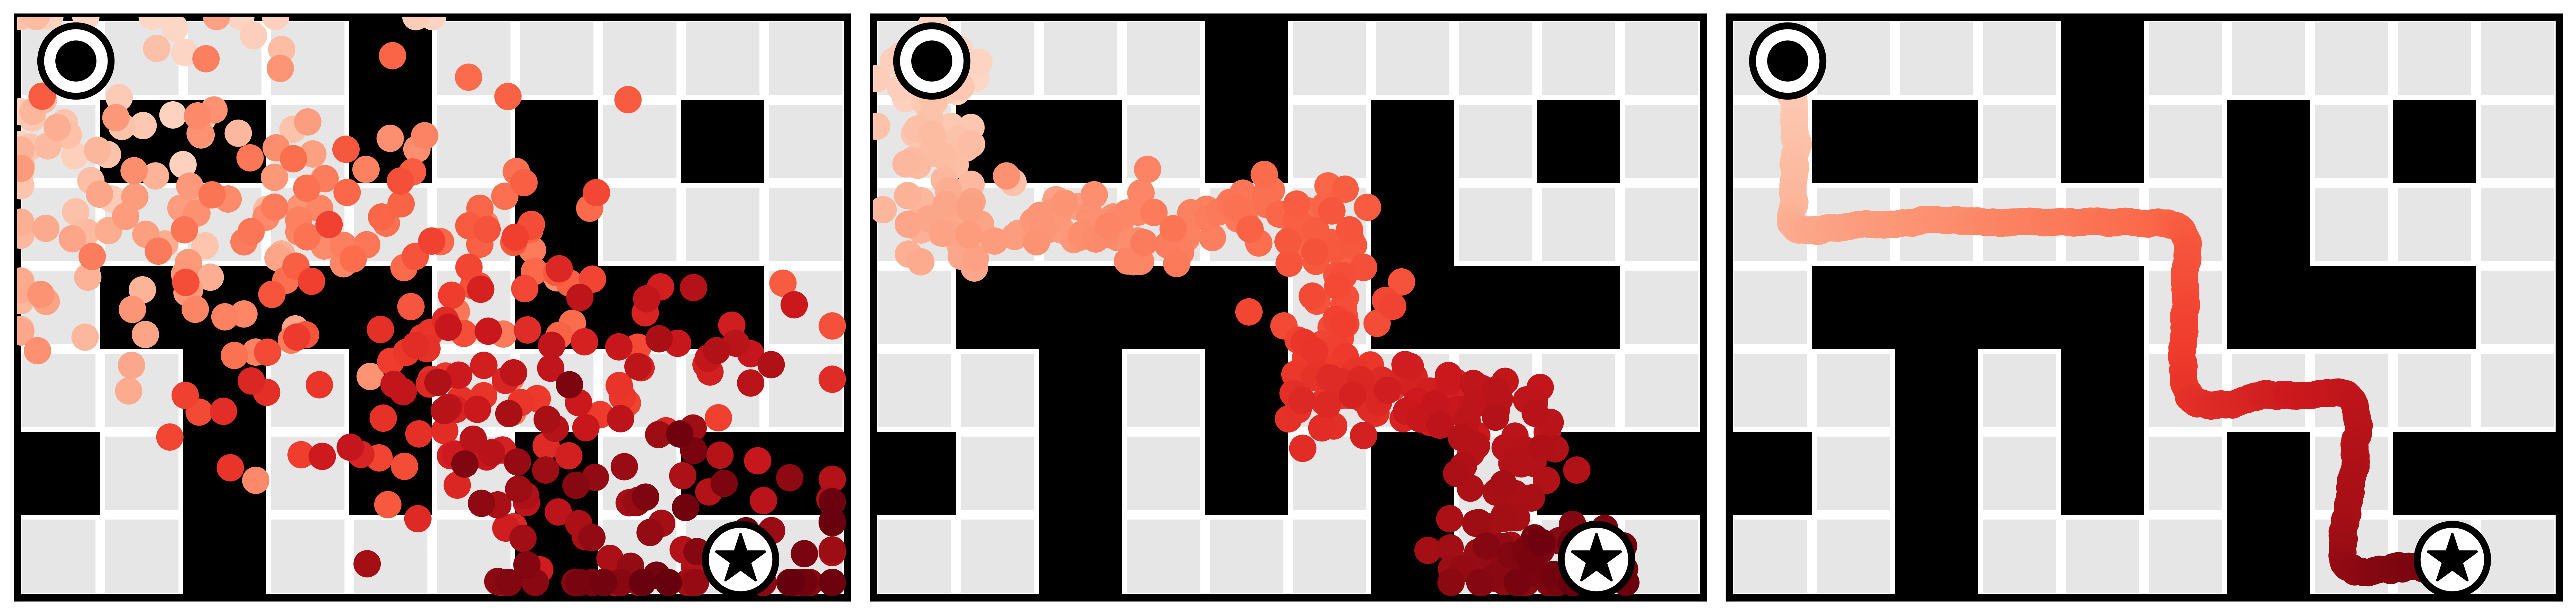
\includegraphics[width=0.95\columnwidth,trim={.03cm 0 .03cm 0},clip]{images/maze2d/maze2d-large-v1.png} \\
\end{flushright}
\begin{centering}
    \raisebox{.3\height}{denoising}~~
    \tikz \draw [-{Computer Modern Rightarrow[length=2mm, width=3mm]}, line width=.3mm] (0,0) -- (3,0); \\
    % \tikz \draw [-{Straight Barb[length=2mm, width=3mm]}, line width=.3mm] (0,0) -- (3,0); \\
\end{centering}
% \vspace{-4pt}
\caption{
    % \small
    \textbf{(Planning as inpainting)}
    Plans are generated in the Maze2D environment by sampling trajectories consistent with a specified start 
    \protect{\raisebox{-.05cm}{
\includegraphics[height=.35cm]{images/maze2d/mark_start_crop.png}}}
    and goal
    \protect{\raisebox{-.05cm}{
\includegraphics[height=.35cm]{images/maze2d/mark_goal_crop.png}}}
    condition.
    The remaining states are ``inpainted'' by the denoising process.
}
% \vspace{-.65cm}
\label{fig:maze2d}
\end{figure}

\definecolor{tblue}{HTML}{1F77B4}
\definecolor{tred}{HTML}{FF6961}
\definecolor{tgreen}{HTML}{429E9D}
\definecolor{thighlight}{HTML}{000000}
\newcolumntype{P}{>{\raggedleft\arraybackslash}X}
\begin{table*}[hb!]
\centering
\small
\begin{tabularx}{\textwidth}{llPPPPPPPPr}
\toprule
\multicolumn{1}{r}{\bf \color{black} Dataset} & \multicolumn{1}{r}{\bf \color{black} Environment} & \multicolumn{1}{r}{\bf \color{black} BC} & \multicolumn{1}{r}{\bf \color{black} CQL} & \multicolumn{1}{r}{\bf \color{black} IQL} & \multicolumn{1}{r}{\bf \color{black} DT} & \multicolumn{1}{r}{\bf \color{black} TT} & \multicolumn{1}{r}{\bf \color{black} MOPO} & \multicolumn{1}{r}{\bf \color{black} MOReL} & \multicolumn{1}{r}{\bf \color{black} MBOP} & \multicolumn{1}{r}{\bf \color{black} Diffuser} \\ 
\midrule
Medium-Expert & HalfCheetah & $55.2$ & $91.6$ & $86.7$ & $86.8$ & $95.0$ & $63.3$ & $53.3$ & $\textbf{\color{thighlight}105.9}$ & $88.9$ \scriptsize{\raisebox{1pt}{$\pm 0.3$}} \\ 
Medium-Expert & Hopper & $52.5$ & $\textbf{\color{thighlight}105.4}$ & $91.5$ & $\textbf{\color{thighlight}107.6}$ & $\textbf{\color{thighlight}110.0}$ & $23.7$ & $\textbf{\color{thighlight}108.7}$ & $55.1$ & $103.3$ \scriptsize{\raisebox{1pt}{$\pm 1.3$}} \\ 
Medium-Expert & Walker2d & $\textbf{\color{thighlight}107.5}$ & $\textbf{\color{thighlight}108.8}$ & $\textbf{\color{thighlight}109.6}$ & $\textbf{\color{thighlight}108.1}$ & $101.9$ & $44.6$ & $95.6$ & $70.2$ & $\textbf{\color{thighlight}106.9}$ \scriptsize{\raisebox{1pt}{$\pm 0.2$}} \\ 
\midrule
Medium & HalfCheetah & $42.6$ & $44.0$ & $\textbf{\color{thighlight}47.4}$ & $42.6$ & $\textbf{\color{thighlight}46.9}$ & $42.3$ & $42.1$ & $44.6$ & $42.8$ \scriptsize{\raisebox{1pt}{$\pm 0.3$}} \\ 
Medium & Hopper & $52.9$ & $58.5$ & $66.3$ & $67.6$ & $61.1$ & $28.0$ & $\textbf{\color{thighlight}95.4}$ & $48.8$ & $74.3$ \scriptsize{\raisebox{1pt}{$\pm 1.4$}} \\ 
Medium & Walker2d & $75.3$ & $72.5$ & $\textbf{\color{thighlight}78.3}$ & $74.0$ & $\textbf{\color{thighlight}79.0}$ & $17.8$ & $\textbf{\color{thighlight}77.8}$ & $41.0$ & $\textbf{\color{thighlight}79.6}$ \scriptsize{\raisebox{1pt}{$\pm 0.55$}} \\ 
\midrule
Medium-Replay & HalfCheetah & $36.6$ & $45.5$ & $44.2$ & $36.6$ & $41.9$ & $\textbf{\color{thighlight}53.1}$ & $40.2$ & $42.3$ & $37.7$ \scriptsize{\raisebox{1pt}{$\pm 0.5$}} \\ 
Medium-Replay & Hopper & $18.1$ & $\textbf{\color{thighlight}95.0}$ & $\textbf{\color{thighlight}94.7}$ & $82.7$ & $\textbf{\color{thighlight}91.5}$ & $67.5$ & $\textbf{\color{thighlight}93.6}$ & $12.4$ & $\textbf{\color{thighlight}93.6}$ \scriptsize{\raisebox{1pt}{$\pm 0.4$}} \\ 
Medium-Replay & Walker2d & $26.0$ & $77.2$ & $73.9$ & $66.6$ & $\textbf{\color{thighlight}82.6}$ & $39.0$ & $49.8$ & $9.7$ & $70.6$ \scriptsize{\raisebox{1pt}{$\pm 1.6$}} \\ 
\midrule
\multicolumn{2}{c}{\bf Average} & 51.9 & \textbf{\color{thighlight}77.6} & \textbf{\color{thighlight}77.0} & 74.7 & \textbf{\color{thighlight}78.9} & 42.1 & 72.9 & 47.8 & \textbf{\color{thighlight}77.5} \hspace{.6cm} \\ 
\bottomrule
\end{tabularx}
\vspace{-.0cm}
\caption{
    \textbf{(Offline reinforcement learning)}
    The performance of \method{} and a variety of prior algorithms on the D4RL locomotion benchmark \citep{fu2020d4rl}.
    Results for \method{} correspond to the mean and standard error over 150 planning seeds. We detail the sources for the performance of prior methods in Appendix~\ref{app:d4rl_sources}. Following \citet{kostrikov2021implicit}, we emphasize in bold scores within 5 percent of the maximum per task ($\ge 0.95 \cdot \text{max}$).
}
\label{table:locomotion}
\end{table*}


\vspace{-.2cm}
\subsection{Test-time Flexibility}
\label{sec:blocks}

In order to evaluate the ability to generalize to new test-time goals, we construct a suite of block stacking tasks with three settings: \textbf{(1)} {\it Unconditional Stacking}, for which the task is to build a block tower as tall as possible; \textbf{(2)} {\it Conditional Stacking}, for which the task is to construct a block tower with a specified order of blocks, and \textbf{(3)} {\it Rearrangement}, for which the task is to match a set of reference blocks' locations in a novel arrangement.
We train all methods on 10000 trajectories from demonstrations generated by PDDLStream \citep{garrett2020pddlstream}; rewards are equal to one upon successful stack placements and zero otherwise.
These block stacking are challenging diagnostics of test-time flexibility;
in the course of executing a partial stack for a randomized goal, a controller will venture into novel states not included in the training configuration.

We use one trained \method for all block-stacking tasks, only modifying the perturbation function $h(\btau{})$ between settings.
In the {\it Unconditional Stacking} task, we directly sample from the unperturbed denoising process $p_\theta(\btau{})$ to emulate the PDDLStream controller.
In the {\it Conditional Stacking} and {\it Rearrangement} tasks, we compose two perturbation functions $h(\btau{})$ to bias the sampled trajectories: the first maximizes the likelihood of the trajectory's final state matching the goal configuration, and the second enforces a contact constraint between the end effector and a cube during stacking motions.
(See Appendix~\ref{app:stacking_costs} for details.)

\begin{figure}[t]
    \centering
    \small
    \begin{tabular}{@{\extracolsep{\fill}}lrrr}
    \toprule
    \multicolumn{1}{c}{\bf Environment} & \multicolumn{1}{c}{\bf ~~~~~BCQ~} &
        \multicolumn{1}{c}{\bf ~~~~~CQL~} &
        \multicolumn{1}{c}{\bf ~~\method} \\
    \midrule
    Unconditional Stacking & $0.0$ & $24.4$ & ~\highlight{\color{highlight}58.7} \scriptsize{\raisebox{1pt}{$\pm 2.5$}}
         \\ 
    Conditional Stacking & 0.0  & 0.0 & \highlight{\color{highlight}45.6} \scriptsize{\raisebox{1pt}{$\pm 3.1$}}
         \\ 
    Rearrangement & 0.0  & 0.0 & \highlight{\color{highlight}58.9} \scriptsize{\raisebox{1pt}{$\pm 3.4$}} \\ 
    \midrule
    \multicolumn{1}{c}{\bf Average} & 0.0  & 8.1 & \highlight{\color{highlight}54.4~~} \hspace{.44cm} \\ 
    \bottomrule
    \end{tabular}
    % \vspace{.2cm}
    \captionof{table}{
    % \small
    % \caption{
    \textbf{(Test-time flexibility)}
    Performance of BCQ, CQL, and \method on block stacking tasks.
    A score of 100 corresponds to a perfectly executed stack; 0 is that of a random policy.
    }
    \label{table:blocks}
    \vspace{-.6cm}
\end{figure}

We compare with two prior model-free offline reinforcement learning algorithms: BCQ \citep{fujimoto2019off} and CQL \citep{kumar2020conservative}, training standard variants for {\it Unconditional Stacking} and goal-conditioned variants for {\it Conditional Stacking} and {\it Rearrangement}.
(Baseline details are provided in Appendix~\ref{app:baselines}.)
Quantitative results are given in Table~\ref{table:blocks}, in which a score of 100 corresponds to a perfect execution of the task.
\method substantially outperforms both prior methods, with the conditional settings requiring flexible behavior generation proving especially difficult for the model-free algorithms.
A visual depiction of an execution by \method is provided in Figure~\ref{fig:blocks}.

\subsection{Offline Reinforcement Learning}
\label{sec:locomotion}
\vspace{-.1cm}
\begin{figure}[t]
    \vspace{-.25cm}
    \centering
    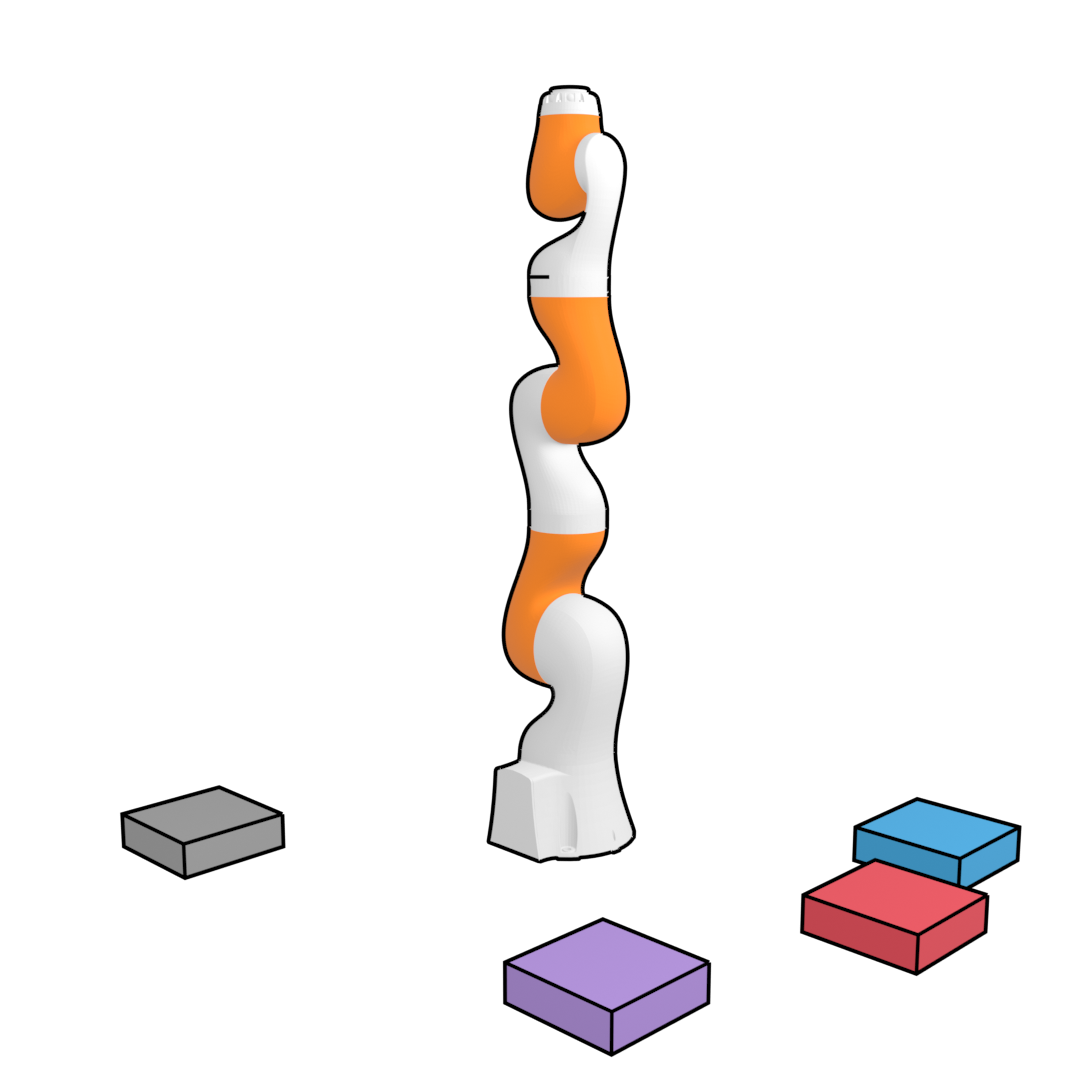
\includegraphics[width=0.45\columnwidth]{images/blocks/blocks_0.png}
    \raisebox{1.7cm}{\hspace{-.1cm}$\rightarrow$}\hspace{.3cm}
    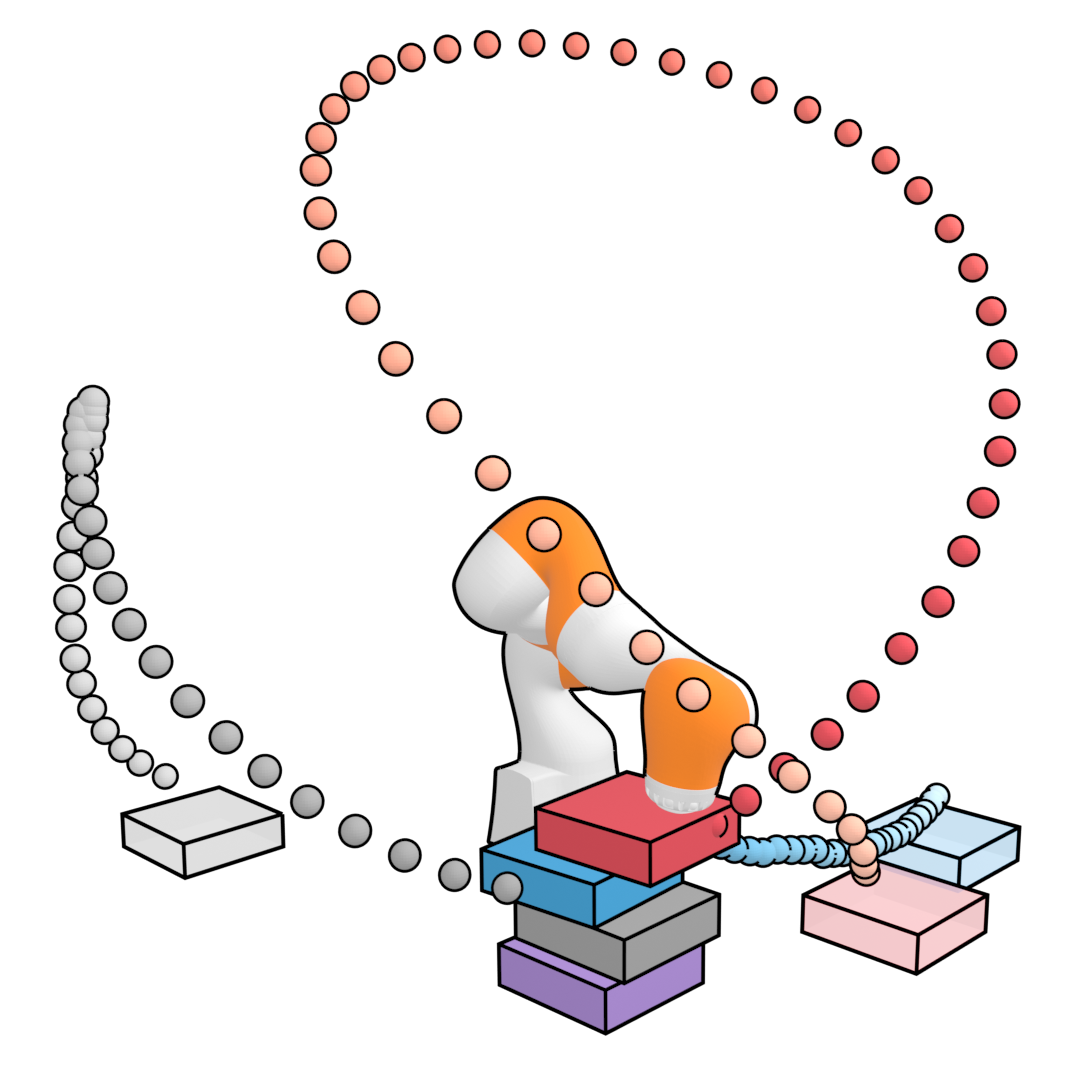
\includegraphics[width=0.45\columnwidth]{images/blocks/blocks_1.png}
    \caption{
        \textbf{(Block stacking)}
        A block stacking sequence executed by \method. This task is best illustrated by videos viewable at
        \href{https://diffusion-planning.github.io/}
        {\texttt{diffusion-planning.github.io}}.
    }
    \label{fig:blocks}
    \vspace{-.3cm}
\end{figure}


Finally, we evaluate the capacity to recover an effective single-task controller from heterogeneous data of varying quality using the D4RL offline locomotion suite \citep{fu2020d4rl}.
We guide the trajectories generated by \method toward high-reward regions using the sampling procedure described in Section~\ref{sec:guided} and condition the trajectories on the current state using the inpainting procedure described in Section~\ref{sec:inpainting}.
The reward predictor $\mathcal{J}_\phi$ is trained on the same trajectories as the diffusion model.

We compare to a variety of prior algorithms spanning other approaches to data-driven control, including the model-free reinforcement learning algorithms CQL \citep{kumar2020conservative} and IQL \citep{kostrikov2021implicit}; return-conditioning approaches like Decision Transformer (DT; \citealt{chen2021decision}); and model-based reinforcement learning approaches including Trajectory Transformer (TT; \citealt{janner2021sequence}), MOPO \citep{yu2020mopo}, MOReL \citep{kidambi2020morel}, and MBOP \citep{argenson2020model}.
In the single-task setting, \method performance comparably to prior algorithms: better than the model-based MOReL and MBOP and return-conditioning DT, but worse than the best offline techniques designed specifically for single-task performance.
% As this setting is one of the most studied in offline reinforcement learning, performances are often within a few percent of each other.
We also investigated a variant using Diffuser as a dynamics model in conventional trajectory optimizers such as MPPI \citep{grady2015mppi}, but found that this combination performed no better than random, suggesting that the effectiveness of Diffuser stems from coupled modeling and planning, and not from improved open-loop predictive accuracy.
%% MJ: The natural question to ask here is "why isn't that included in Table 2?" We struck something of a compromise. It seems worth mentioning that a naïve application of Diffuser + MPPI does not work out of the box, but presenting a column full of 0's will cause avoidable problems from people unfamiliar with the extent of tricks needed to make planning with neural nets work. The reality is that it probably *could* be made to work, it would just require a level of effort and tuning similar to PETS. The compromise is to state it as "we tried this but couldn't get it working".

\begin{figure}
\centering
\begin{minipage}{.05\columnwidth}
\begin{flushleft}
    \raisebox{.2\height}{\rotatebox{90}{denoising}}
    \tikz \draw [-{Computer Modern Rightarrow[length=2mm, width=3mm]}, line width=.3mm] (0,2) -- (0,0); \\
\end{flushleft}
\end{minipage}~~
\begin{minipage}{.9\columnwidth}
\centering
    \vspace{.15cm}
    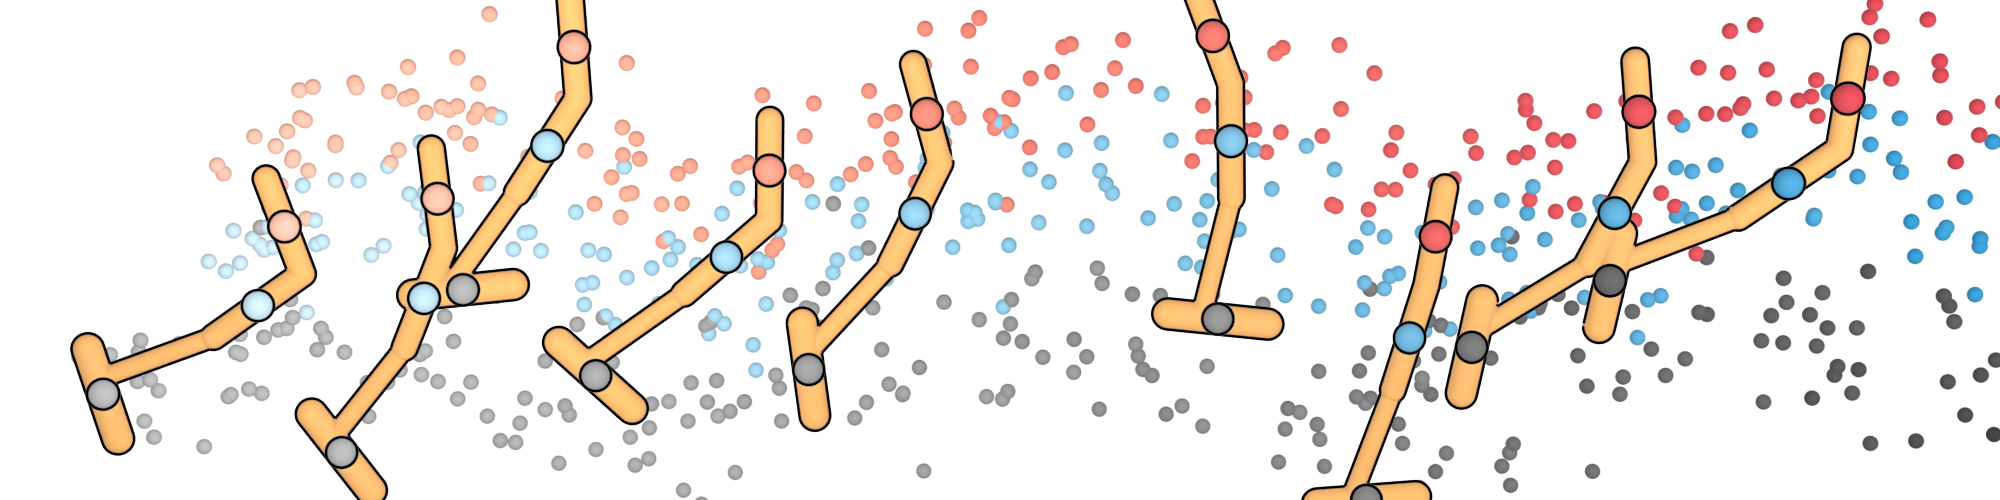
\includegraphics[width=\linewidth]{images/locomotion/merged-hopper-10.png} \\
    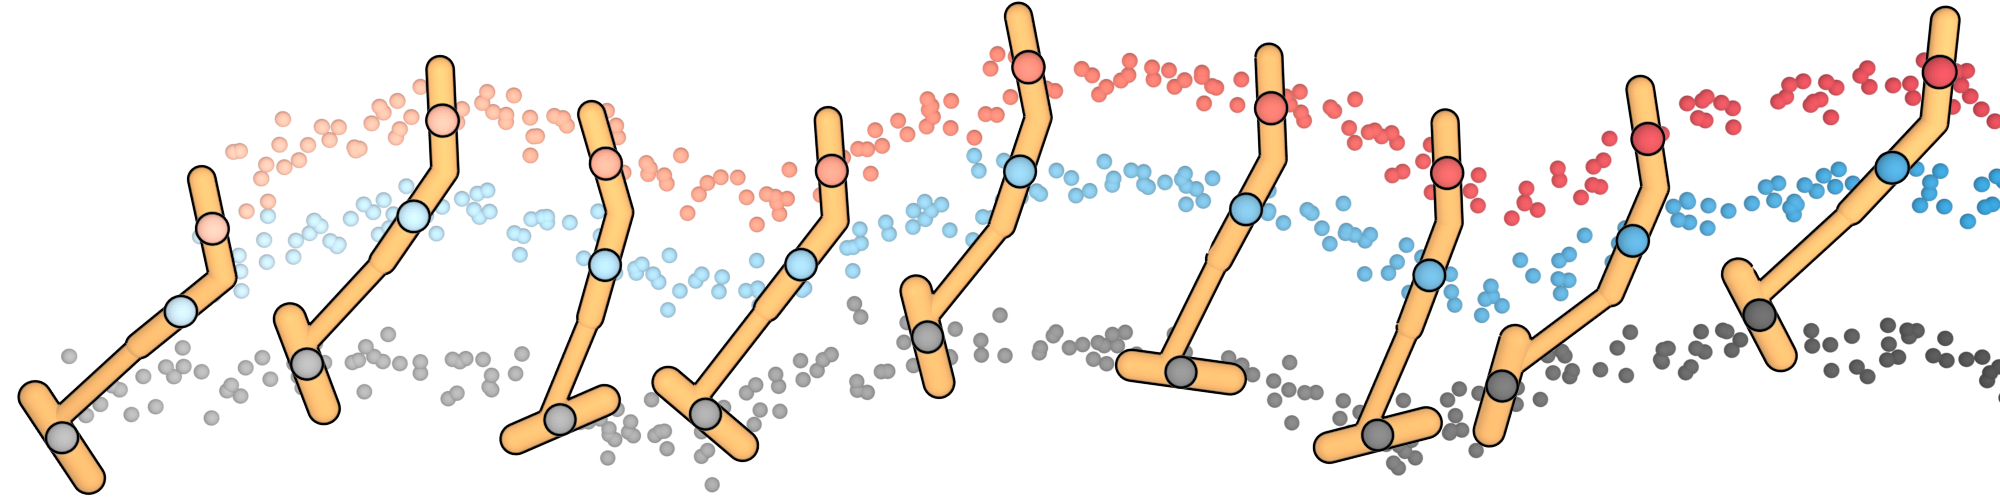
\includegraphics[width=\linewidth]{images/locomotion/merged-hopper-2.png} \\
    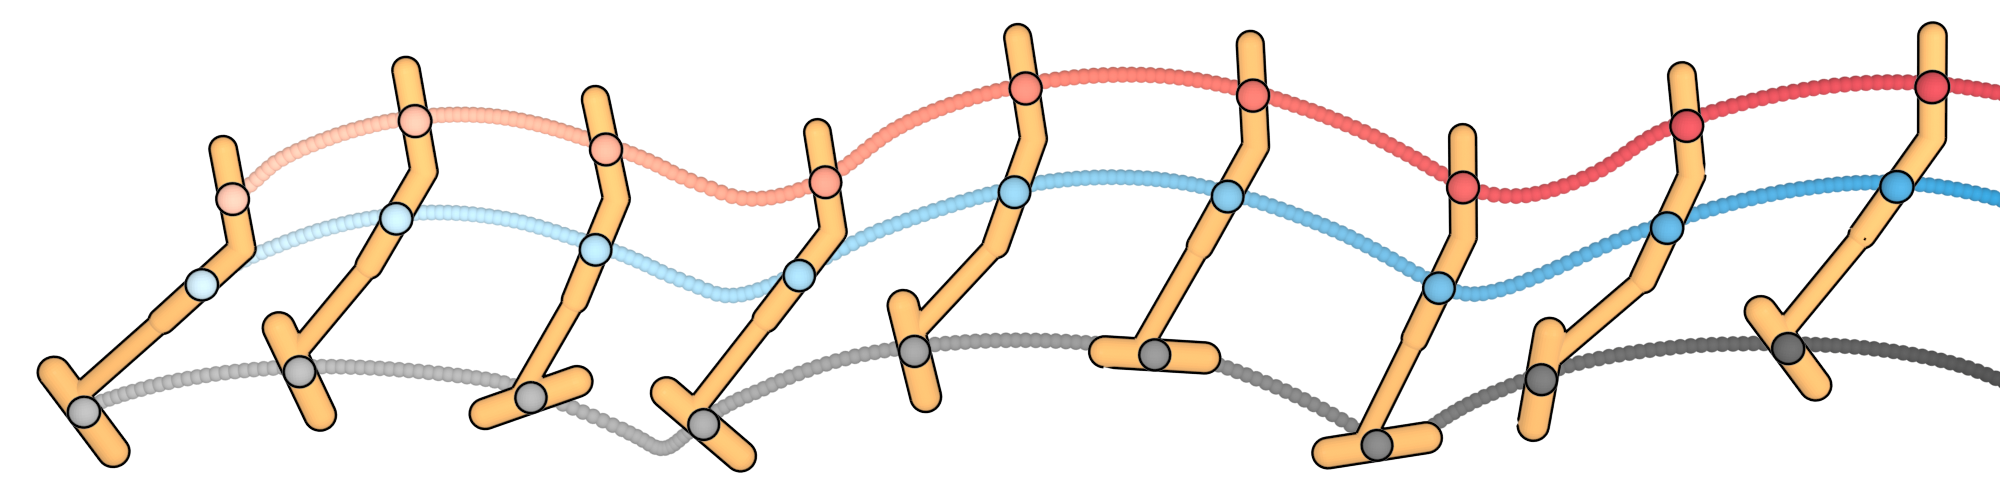
\includegraphics[width=\linewidth]{images/locomotion/merged-hopper-0.png} \\
\end{minipage} \\
\vspace{.3cm}
\hspace{1cm}
\raisebox{.3\height}{planning horizon}~~
\tikz \draw [-{Computer Modern Rightarrow[length=2mm, width=3mm]}, line width=.3mm] (0,0) -- (3,0); \\
\caption{
    \textbf{(Guided sampling)}
    \method generates all timesteps of a plan concurrently, instead of autoregressively, through the denoising process.
}
\vspace{-15pt}
\label{fig:locomotion}
\end{figure}

\subsection{Warm-Starting Diffusion for Faster Planning}

A limitation of \method{} is that individual plans are slow to generate (due to iterative generation). Na\"ively,  as we execute plans open loop, a new plan must be regenerated at each step of execution. To improve execution speed of \method{}, we may further reuse previously generated plans to warm-start generations of subsequent plans. 

To warm-start planning, we may run a limited number of forward diffusion steps from a previously generated plan and then run a corresponding number of denoising steps from this partially noised trajectory to regenerate an updated plan. In \fig{fig:speed}, we illustrate the trade-off between performance and runtime budget as we vary the underlying number of denoising steps used to regenerate each a new plan from 2 to 100. We find that we may reduce the planning budget of our approach markedly with only modest drop in performance.
